\documentclass[11pt,letterpaper]{article}
\setlength{\parindent}{0em}                  %DISTANCIA SANGRÍA
\setlength{\parskip}{0.5em}                  %DISTANCIA ENTRE PÁRRAFOS
\textwidth 6.5in
\textheight 9.in
\oddsidemargin 0in
\headheight 0in



\usepackage{fancybox}
\usepackage[utf8]{inputenc}
\usepackage{epsfig,graphicx}
\usepackage{multicol,pst-plot}
\usepackage{pstricks}
\usepackage{amsmath}
\usepackage{amsfonts}
\usepackage{amssymb}
\usepackage{eucal}
\usepackage[left=2cm,right=2cm,top=2cm,bottom=2cm]{geometry}
\usepackage{txfonts}
\usepackage[english]{babel}
\usepackage[colorlinks]{hyperref}
\usepackage{cancel}
\usepackage{caption}
\usepackage{float}
\usepackage{upgreek}
\usepackage{gensymb}
\usepackage{subfigure}
\usepackage{siunitx}
\usepackage{color}
\usepackage{tikz}
\usepackage{listings}
\usepackage{minted}
\usepackage{mdframed}
\usepackage{natbib}
\usepackage{listings}
\bibliographystyle{mnras}
\setcitestyle{aysep{","}}
\usepackage{multicol}
\renewcommand{\bibpreamble}{\begin{multicols}{2}}
\renewcommand{\bibpostamble}{\end{multicols}}
\setlength{\bibsep}{3pt}

%DEFINICIÓN DE COLORES EXTRAS

\definecolor{codegreen}{rgb}{0,0.6,0}
\definecolor{codegray}{rgb}{0.5,0.5,0.5}
\definecolor{backcolour}{rgb}{0.95,0.95,0.95}
\hypersetup{colorlinks=true,linkcolor=codegreen,citecolor=blue,filecolor=blue,urlcolor=magenta,}

%CONFIGURACIÓN DE LSTLISTINGS PARA CÓDIGOS

\lstset{ %
language=matlab,                % choose the language of the code
basicstyle=\footnotesize,       % the size of the fonts that are used for the code
numbers=left,                   % where to put the line-numbers
numberstyle=\footnotesize,      % the size of the fonts that are used for the line-numbers
stepnumber=1,                   % the step between two line-numbers. If it is 1 each line will be numbered
numbersep=5pt,                  % how far the line-numbers are from the code
backgroundcolor=\color{white},  % choose the background color. You must add \usepackage{color}
showspaces=false,               % show spaces adding particular underscores
showstringspaces=false,         % underline spaces within strings
showtabs=false,                 % show tabs within strings adding particular underscores
frame=single,                   % adds a frame around the code
tabsize=2,                      % sets default tabsize to 2 spaces
captionpos=b,                   % sets the caption-position to bottom
breaklines=true,                % sets automatic line breaking
breakatwhitespace=false,        % sets if automatic breaks should only happen at whitespace
escapeinside={\%*}{*)}          % if you want to add a comment within your code
}
\lstdefinestyle{mystyle}{
	backgroundcolor=\color{backcolour},   
	commentstyle=\color{red},
	keywordstyle=\bfseries\color{magenta},
	numberstyle=\tiny\color{codegray},
	stringstyle=\color{codegreen},
	basicstyle=\footnotesize\ttfamily,
	identifierstyle=\color{blue},
	breakatwhitespace=false,         
	breaklines=true,                 
	captionpos=b,                    
	keepspaces=true,                 
	numbers=left,                    
	numbersep=5pt,                  
	showspaces=false,                
	showstringspaces=false,
	showtabs=false,                  
	tabsize=2
}

\lstset{style=mystyle}


\usemintedstyle{vs}

\pagestyle{empty}


\begin{document}


\usetikzlibrary{positioning}
\tikzset{every picture/.style={line width=0.75pt}}    
\pagestyle{plain}
\begin{flushleft}
Department of Economics \hfill \\
School of Art and Science\\
University of Pennsylvania
\end{flushleft}

\begin{flushright}\vspace{-2cm}

\includegraphics[height=1.5cm]{HW1/LATEX/Attachments/logo.png}
\end{flushright}
 
\begin{center}\vspace{1cm}
\textbf{\large Industrial Organization/Homework 1}\\   %TITULO
\textit{Mahdi Shahrabi} \\\textit{Collaborated with Anna Schetkina}\\                         %NOMBRE

\end{center}
\rule{\linewidth}{0.4mm}

%%%%%%%%%%%%%%%%%%%%%%%%%%%%%%%%%%    Question 1    %%%%%%%%%%%%%%%%%%%%%%%%%%%%%%%
\section{Question 1}
\subsection{(a) & (b) & (c)}

I estimate the equation in problem 1 (a) by including only second lags (specification 1) and by including second and third lags (specification 2). Specification 3 is autocorrelated transmitted shocks without fixed effects (the selected $\rho=0.758$) and specification 4 (the selected $\rho=1.159$) is autocorrelated transmitted shocks with fixed effects.


\begin{figure}[h!]
    \centering
    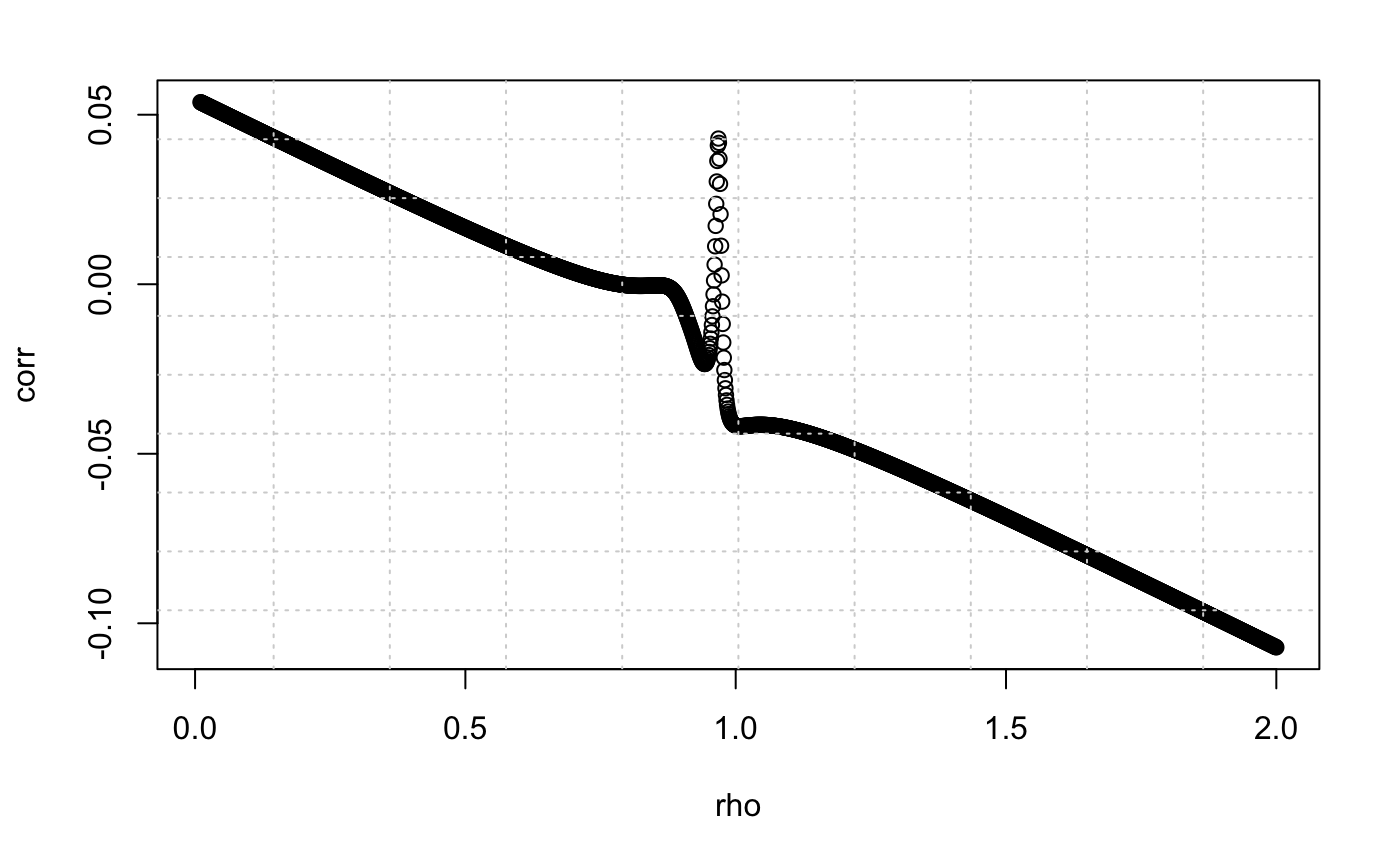
\includegraphics[scale=0.15]{HW2/Attachments/Q1b.png}
    \caption{Moment Condition vs $\rho$ for (b)}
    \label{fig:my_label}
\end{figure}

\begin{figure}[h!]
    \centering
    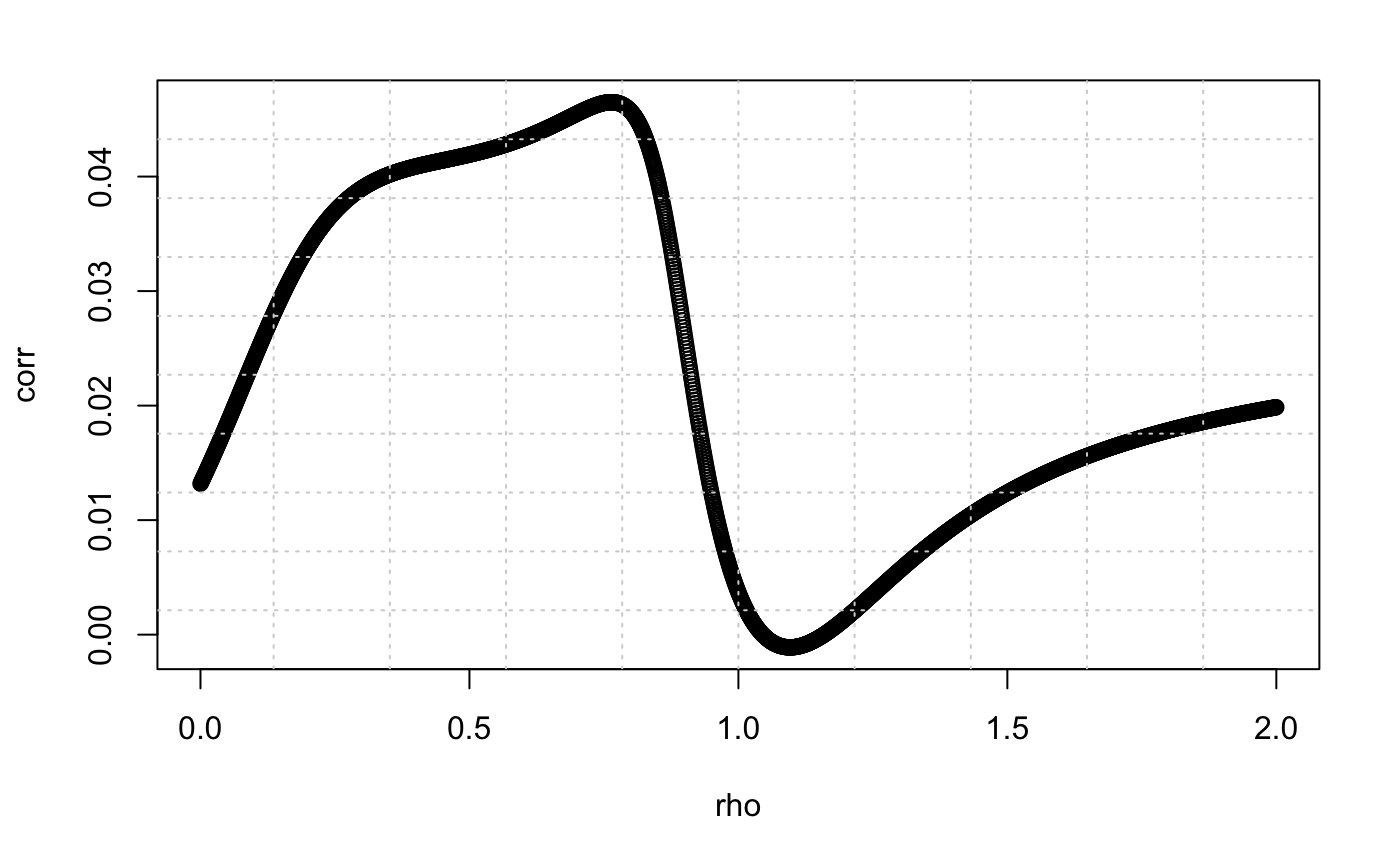
\includegraphics[scale=0.15]{HW2/Attachments/Q1c.png}
    \caption{Moment Condition vs $\rho$ for (c)}
    \label{fig:my_label}
\end{figure}

\begin{table}[h!]
    \centering
    \footnotesize{
    {
\def\sym#1{\ifmmode^{#1}\else\(^{#1}\)\fi}
\begin{tabular}{l*{4}{c}}
\hline\hline
            &\multicolumn{1}{c}{(1)}&\multicolumn{1}{c}{(2)}&\multicolumn{1}{c}{(3)}&\multicolumn{1}{c}{(4)}\\
            &\multicolumn{1}{c}{IV Regressions with 2L}&\multicolumn{1}{c}{IV Regressions with 3L}&\multicolumn{1}{c}{AR Shocks}&\multicolumn{1}{c}{AR Shocks+FE}\\
\hline
lemp        &       0.221         &       0.661         &       0.517\sym{***}&      -1.076         \\
            &      (0.68)         &      (1.85)         &      (3.65)         &     (-0.25)         \\
[1em]
ldnpt       &       0.869\sym{**} &      -0.269         &       0.439\sym{***}&       4.013         \\
            &      (2.78)         &     (-0.68)         &      (4.54)         &      (0.56)         \\
[1em]
ldrst       &      -0.555         &       0.409         &      0.0963         &       0.221         \\
            &     (-1.70)         &      (1.34)         &      (1.32)         &      (0.03)         \\
[1em]
d73         &           0         &           0         &           0         &           0         \\
            &         (.)         &         (.)         &         (.)         &         (.)         \\
[1em]
d78         &           0         &           0         &           0         &           0         \\
            &         (.)         &         (.)         &         (.)         &         (.)         \\
[1em]
d83         &      -0.633\sym{***}&           0         &      -0.390\sym{***}&           0         \\
            &     (-4.46)         &         (.)         &    (-11.21)         &         (.)         \\
[1em]
d88         &           0         &           0         &           0         &           0         \\
            &         (.)         &         (.)         &         (.)         &         (.)         \\
[1em]
d357\_73     &           0         &           0         &           0         &           0         \\
            &         (.)         &         (.)         &         (.)         &         (.)         \\
[1em]
d357\_78     &           0         &           0         &           0         &           0         \\
            &         (.)         &         (.)         &         (.)         &         (.)         \\
[1em]
d357\_83     &       1.471\sym{***}&           0         &       0.853\sym{***}&           0         \\
            &     (13.80)         &         (.)         &     (16.92)         &         (.)         \\
[1em]
d357\_88     &       1.087\sym{***}&       0.903\sym{***}&       0.810\sym{***}&      -0.798         \\
            &     (10.69)         &      (8.71)         &     (15.09)         &     (-0.75)         \\
[1em]
\_cons      &       0.474\sym{***}&       0.161         &       0.820\sym{***}&       1.959         \\
            &      (4.66)         &      (1.66)         &     (10.55)         &      (0.68)         \\
\hline
\(N\)       &         682         &         214         &         682         &         214         \\
\hline\hline
\multicolumn{5}{l}{\footnotesize \textit{t} statistics in parentheses}\\
\multicolumn{5}{l}{\footnotesize \sym{*} \(p<0.05\), \sym{**} \(p<0.01\), \sym{***} \(p<0.001\)}\\
\end{tabular}
}

    }
    \caption{Question 1}
    \label{tab:my_label}
\end{table}

\subsection{(d)}

As we can see from Table 1, specifications (1) and (2) do not make much sense: in specification (1), the coefficient on R\&D capital is negative, while in specification (2) the coefficient on capital is negative. The first stage of both these regressions suggests that the instruments might be weak: the F-statistic of the first stage is around 10 in specification (1) and much lower than 10 in specification (2).

The results of specification (3) seem much more reasonable compared to specifications (1) and (2), suggesting that the assumption of no autocorrelation in the transmitted shock is restrictive. The estimated autocorrelation is $\rho=0.758$, which is a high coefficient, so ignoring it results in a seriously biased estimates.

The results of specification (4) are also not reasonable: they suggest that nothing is significant. Including fixed effects forces us to (i) use only a balanced panel for estimation, reducing the sample size threefold, and (ii) use higher-order lags for estimation which makes them weaker instruments. That is, on this sample, accounting for fixed effects creates more problems than it solves.


%%%%%%%%%%%%%%%%%%%%%%%%%%%%%%%%%%    Question 2    %%%%%%%%%%%%%%%%%%%%%%%%%%%%%%%
\newpage
\section{Question 2}


\subsection{(a) \& (b) \& (c)}



\begin{table}[h]
\parbox{.45\linewidth}{
    \centering
    \footnotesize{
    {
\def\sym#1{\ifmmode^{#1}\else\(^{#1}\)\fi}
\begin{tabular}{l*{3}{c}}
\hline\hline
            &\multicolumn{1}{c}{(1)}&\multicolumn{1}{c}{(2)}&\multicolumn{1}{c}{(3)}\\
            &\multicolumn{1}{c}{h^}&\multicolumn{1}{c}{P^}&\multicolumn{1}{c}{h^ & P^}\\
\hline
beta2       &                     &                     &                     \\
\_cons      &       0.379\sym{***}&       0.403\sym{***}&       0.384\sym{***}\\
            &    (125.92)         &     (92.99)         &    (133.29)         \\
\hline
beta3       &                     &                     &                     \\
\_cons      &      0.0414\sym{***}&      0.0327\sym{**} &      0.0706\sym{***}\\
            &     (12.56)         &      (3.07)         &     (13.71)         \\
\hline
b1          &                     &                     &                     \\
\_cons      &       1.426\sym{***}&       9.903\sym{***}&      -0.628\sym{***}\\
            &     (71.99)         &    (163.09)         &     (-5.51)         \\
\hline
b2          &                     &                     &                     \\
\_cons      &      -0.131\sym{***}&      -7.394\sym{***}&       0.272\sym{**} \\
            &    (-21.72)         &    (-49.78)         &      (3.03)         \\
\hline
b3          &                     &                     &                     \\
\_cons      &                     &                     &       1.637\sym{***}\\
            &                     &                     &     (54.08)         \\
\hline
b4          &                     &                     &                     \\
\_cons      &                     &                     &      -0.174\sym{***}\\
            &                     &                     &    (-25.64)         \\
\hline
\(N\)       &        1502         &        1502         &        1502         \\
\hline\hline
\multicolumn{4}{l}{\footnotesize \textit{t} statistics in parentheses}\\
\multicolumn{4}{l}{\footnotesize \sym{*} \(p<0.05\), \sym{**} \(p<0.01\), \sym{***} \(p<0.001\)}\\
\end{tabular}
}

    }
    \caption{NLSS}
    \label{tab:my_label}
    }
    \quad
\parbox{.45\linewidth}{
    \centering
    \footnotesize{
    {
\def\sym#1{\ifmmode^{#1}\else\(^{#1}\)\fi}
\begin{tabular}{l*{1}{c}}
\hline\hline
            &\multicolumn{1}{c}{(1)}\\
            &\multicolumn{1}{c}{lemp and dummies}\\
\hline
lemp        &       0.584\sym{***}\\
            &     (44.18)         \\
[1em]
d73         &      -0.169\sym{***}\\
            &     (-7.53)         \\
[1em]
d78         &      -0.153\sym{***}\\
            &     (-7.35)         \\
[1em]
d83         &      -0.220\sym{***}\\
            &    (-10.17)         \\
[1em]
d88         &           0         \\
            &         (.)         \\
[1em]
d357\_73     &      -3.245\sym{***}\\
            &    (-38.88)         \\
[1em]
d357\_78     &      -2.037\sym{***}\\
            &    (-35.87)         \\
[1em]
d357\_83     &      -0.757\sym{***}\\
            &    (-13.16)         \\
[1em]
d357\_88     &       0.408\sym{***}\\
[1em]
\_cons      &       3.661\sym{***}\\
            &     (65.96)         \\
\hline
\(N\)       &        2971         \\
\hline\hline
\multicolumn{2}{l}{\footnotesize \textit{t} statistics in parentheses}\\
\multicolumn{2}{l}{\footnotesize \sym{*} \(p<0.05\), \sym{**} \(p<0.01\), \sym{***} \(p<0.001\)}\\
\end{tabular}
}

    }
    \caption{For lemp and Dummies}
    \label{tab:my_label}
}

\end{table}

\subsection{(d)}
\
As we can see from Table 2, the results do not change much between specifications. This suggests that the additional information brought from exit decisions can substitute for the usual inversion of the investment decision function. Moreover, the results in Tables 2 and 3 are reasonable: the coefficient on labor is 0.58, and the coefficient on capital is around 0.38. These results are very similar to the results from specification (3) from Problem 1 — the specification that modeled transmitted shocks as AR processes. We can conclude that allowing for a more general process than AR does not add much. And as we have seen in problem 1, allowing for fixed effects even creates additional problems.




%%%%%%%%%%%%%%%%%%%%%%%%%%%%%%%%%%    Question 3    %%%%%%%%%%%%%%%%%%%%%%%%%%%%%%%
\newpage
\section{Question 3}
\subsection{Regression Results}

\begin{table}[h]
    \centering
    \small
    {
\def\sym#1{\ifmmode^{#1}\else\(^{#1}\)\fi}
\begin{tabular}{l*{3}{c}}
\hline\hline
            &\multicolumn{1}{c}{(1)}&\multicolumn{1}{c}{(2)}&\multicolumn{1}{c}{(3)}\\
            &\multicolumn{1}{c}{1st diff}&\multicolumn{1}{c}{2nd diff}&\multicolumn{1}{c}{3rd diff}\\
\hline
lemp        &       0.689\sym{***}&       0.687\sym{***}&       0.710\sym{***}\\
            &     (23.28)         &     (17.71)         &     (12.32)         \\
[1em]
ldnpt       &       0.162\sym{***}&       0.177\sym{***}&       0.196\sym{***}\\
            &      (6.12)         &      (5.40)         &      (4.13)         \\
[1em]
ldrst       &      0.0604         &     -0.0715         &     -0.0893         \\
            &      (1.95)         &     (-1.34)         &     (-1.02)         \\
[1em]
d73         &           0         &           0         &           0         \\
            &         (.)         &         (.)         &         (.)         \\
[1em]
d78         &     -0.0334\sym{**} &       0.142\sym{***}&           0         \\
            &     (-2.99)         &     (12.37)         &         (.)         \\
[1em]
d83         &      -0.171\sym{***}&           0         &           0         \\
            &    (-13.84)         &         (.)         &         (.)         \\
[1em]
d88         &           0         &           0         &           0         \\
            &         (.)         &         (.)         &         (.)         \\
[1em]
d357\_73     &           0         &           0         &           0         \\
            &         (.)         &         (.)         &         (.)         \\
[1em]
d357\_78     &       1.145\sym{***}&     -0.0154         &      -0.204\sym{***}\\
            &     (18.66)         &     (-0.22)         &     (-3.69)         \\
[1em]
d357\_83     &       2.505\sym{***}&       0.196\sym{**} &           0         \\
            &     (28.40)         &      (2.84)         &         (.)         \\
[1em]
d357\_88     &       3.464\sym{***}&           0         &           0         \\
            &     (31.89)         &         (.)         &         (.)         \\
[1em]
\_cons      &      0.0920\sym{***}&       0.181\sym{***}&       0.428\sym{***}\\
            &      (9.69)         &     (10.74)         &      (9.44)         \\
\hline
\(N\)       &         642         &         428         &         214         \\
\hline\hline
\multicolumn{4}{l}{\footnotesize \textit{t} statistics in parentheses}\\
\multicolumn{4}{l}{\footnotesize \sym{*} \(p<0.05\), \sym{**} \(p<0.01\), \sym{***} \(p<0.001\)}\\
\end{tabular}
}

    \caption{Regression Results for Difference Model}
    \label{tab:my_label}
\end{table}

For models (1), (2), and (3), variables on left columns respectively reflect first, second, third differences.

\subsection{What does it say about measurement error?}
From Griliches and Hausman (1986), if variables are serially correlated, and there is a measurement error in the inputs, the shorter-difference estimates will be biased toward zero. The fact that the 5, 10, and 15 years difference estimators report different coefficients tells us that there probably was a measurement error in the inputs in lemp and ldnpt. Also

%%%%%%%%%%%%%%%%%%%%%%%%%%%%%%%%%%    Question 4    %%%%%%%%%%%%%%%%%%%%%%%%%%%%%%%
\newpage
\section{Question 4}
\subsection{Unbalanced and at least Two observations regressions}

\begin{table}[h]
\parbox{.45\linewidth}{
    \centering
    \small
    {
\def\sym#1{\ifmmode^{#1}\else\(^{#1}\)\fi}
\begin{tabular}{l*{2}{c}}
\hline\hline
            &\multicolumn{1}{c}{(1)}&\multicolumn{1}{c}{(2)}\\
            &\multicolumn{1}{c}{Total}&\multicolumn{1}{c}{1st diff}\\
\hline
lemp        &       0.578\sym{***}&       0.740\sym{***}\\
            &     (45.87)         &     (39.96)         \\
[1em]
ldnpt       &       0.372\sym{***}&       0.116\sym{***}\\
            &     (40.08)         &      (7.38)         \\
[1em]
ldrst       &      0.0380\sym{***}&      0.0414\sym{*}  \\
            &      (5.36)         &      (2.43)         \\
[1em]
d73         &      -0.192\sym{***}&           0         \\
            &     (-8.37)         &         (.)         \\
[1em]
d78         &      -0.169\sym{***}&     -0.0453\sym{***}\\
            &     (-7.98)         &     (-5.50)         \\
[1em]
d83         &      -0.267\sym{***}&      -0.167\sym{***}\\
            &    (-12.41)         &    (-18.67)         \\
[1em]
d88         &           0         &           0         \\
            &         (.)         &         (.)         \\
[1em]
d357\_73     &      -3.211\sym{***}&           0         \\
            &    (-37.54)         &         (.)         \\
[1em]
d357\_78     &      -1.973\sym{***}&       1.134\sym{***}\\
            &    (-34.32)         &     (23.41)         \\
[1em]
d357\_83     &      -0.689\sym{***}&       2.453\sym{***}\\
            &    (-11.80)         &     (38.87)         \\
[1em]
d357\_88     &       0.466\sym{***}&       3.517\sym{***}\\
            &      (9.97)         &     (47.44)         \\
[1em]
\_cons      &       3.365\sym{***}&      0.0915\sym{***}\\
            &     (94.11)         &     (13.43)         \\
\hline
\(N\)       &        2971         &        1502         \\
\hline\hline
\multicolumn{3}{l}{\footnotesize \textit{t} statistics in parentheses}\\
\multicolumn{3}{l}{\footnotesize \sym{*} \(p<0.05\), \sym{**} \(p<0.01\), \sym{***} \(p<0.001\)}\\
\end{tabular}
}

    \caption{Unbalanced Panel(All)}
    \label{tab:my_label}
    }
    \quad
    \parbox{.45\linewidth}{
    \centering
    \small
    {
\def\sym#1{\ifmmode^{#1}\else\(^{#1}\)\fi}
\begin{tabular}{l*{2}{c}}
\hline\hline
            &\multicolumn{1}{c}{(1)}&\multicolumn{1}{c}{(2)}\\
            &\multicolumn{1}{c}{Total}&\multicolumn{1}{c}{1st diff}\\
\hline
lemp        &       0.541\sym{***}&       0.740\sym{***}\\
            &     (39.41)         &     (39.96)         \\
[1em]
ldnpt       &       0.392\sym{***}&       0.116\sym{***}\\
            &     (39.40)         &      (7.38)         \\
[1em]
ldrst       &      0.0534\sym{***}&      0.0414\sym{*}  \\
            &      (6.73)         &      (2.43)         \\
[1em]
d73         &      -0.181\sym{***}&           0         \\
            &     (-7.26)         &         (.)         \\
[1em]
d78         &      -0.149\sym{***}&     -0.0453\sym{***}\\
            &     (-6.51)         &     (-5.50)         \\
[1em]
d83         &      -0.267\sym{***}&      -0.167\sym{***}\\
            &    (-11.62)         &    (-18.67)         \\
[1em]
d88         &           0         &           0         \\
            &         (.)         &         (.)         \\
[1em]
d357\_73     &      -3.221\sym{***}&           0         \\
            &    (-38.07)         &         (.)         \\
[1em]
d357\_78     &      -2.025\sym{***}&       1.134\sym{***}\\
            &    (-32.25)         &     (23.41)         \\
[1em]
d357\_83     &      -0.683\sym{***}&       2.453\sym{***}\\
            &    (-11.96)         &     (38.87)         \\
[1em]
d357\_88     &       0.343\sym{***}&       3.517\sym{***}\\
            &      (5.36)         &     (47.44)         \\
[1em]
\_cons      &       3.264\sym{***}&      0.0915\sym{***}\\
            &     (83.23)         &     (13.43)         \\
\hline
\(N\)       &        2440         &        1502         \\
\hline\hline
\multicolumn{3}{l}{\footnotesize \textit{t} statistics in parentheses}\\
\multicolumn{3}{l}{\footnotesize \sym{*} \(p<0.05\), \sym{**} \(p<0.01\), \sym{***} \(p<0.001\)}\\
\end{tabular}
}

    \caption{Firms with at least two observations}
    \label{tab:my_label}
    }
\end{table}


The coefficient of labor is higher when estimated on the whole sample compared to the balanced subpanel estimate, while the coefficient on capital is lower. These results indicate that the companies in the balanced subpanel (i.e., surviving for 15 years) are fundamentally different from the companies in the total sample, which confirms the insights from the descriptive statistics. One possibility is that shorter-living companies are more labor-intensive and do not have time to acquire much capital, which shifts the estimates toward a higher labor coefficient and a lower capital coefficient when they are included in the estimation.\\

\subsection{Probit}

\begin{table}[h]
\parbox{.45\linewidth}{
    \centering
    \small
    {
\def\sym#1{\ifmmode^{#1}\else\(^{#1}\)\fi}
\begin{tabular}{l*{1}{c}}
\hline\hline
            &\multicolumn{1}{c}{(1)}\\
            &\multicolumn{1}{c}{probit}\\
\hline
next\_period &                     \\
ldnpt       &      -0.183\sym{***}\\
            &     (-4.51)         \\
[1em]
ldrst       &       0.172\sym{***}\\
            &      (6.71)         \\
[1em]
ldinv       &       0.193\sym{***}\\
            &      (4.65)         \\
[1em]
\_cons      &       0.272\sym{**} \\
            &      (2.99)         \\
\hline
\(N\)       &        2285         \\
\hline\hline
\multicolumn{2}{l}{\footnotesize \textit{t} statistics in parentheses}\\
\multicolumn{2}{l}{\footnotesize \sym{*} \(p<0.05\), \sym{**} \(p<0.01\), \sym{***} \(p<0.001\)}\\
\end{tabular}
}

    \caption{Regression Results after using probit results}
    \label{tab:my_label}
}
\quad
\parbox{.45\linewidth}{
    \centering
    \small
    {
\def\sym#1{\ifmmode^{#1}\else\(^{#1}\)\fi}
\begin{tabular}{l*{2}{c}}
\hline\hline
            &\multicolumn{1}{c}{(1)}&\multicolumn{1}{c}{(2)}\\
            &\multicolumn{1}{c}{Total}&\multicolumn{1}{c}{1st diff}\\
\hline
lemp        &       0.526\sym{***}&       0.710\sym{***}\\
            &     (37.99)         &     (37.06)         \\
[1em]
ldnpt       &       0.403\sym{***}&       0.136\sym{***}\\
            &     (40.00)         &      (8.49)         \\
[1em]
ldrst       &      0.0169         &      0.0227         \\
            &      (1.66)         &      (1.32)         \\
[1em]
d73         &      -0.169\sym{***}&           0         \\
            &     (-6.81)         &         (.)         \\
[1em]
d78         &      -0.139\sym{***}&     -0.0385\sym{***}\\
            &     (-6.09)         &     (-4.67)         \\
[1em]
d83         &      -0.250\sym{***}&      -0.151\sym{***}\\
            &    (-10.86)         &    (-16.24)         \\
[1em]
d88         &           0         &           0         \\
            &         (.)         &         (.)         \\
[1em]
d357\_73     &      -3.259\sym{***}&           0         \\
            &    (-38.64)         &         (.)         \\
[1em]
d357\_78     &      -2.064\sym{***}&       1.120\sym{***}\\
            &    (-32.89)         &     (23.30)         \\
[1em]
d357\_83     &      -0.720\sym{***}&       2.433\sym{***}\\
            &    (-12.60)         &     (38.86)         \\
[1em]
d357\_88     &       0.294\sym{***}&       3.472\sym{***}\\
            &      (4.57)         &     (46.98)         \\
[1em]
inv\_mills   &      0.0674\sym{***}&      0.0692\sym{***}\\
            &      (5.68)         &      (5.39)         \\
[1em]
\_cons      &       3.191\sym{***}&      0.0853\sym{***}\\
            &     (77.74)         &     (12.44)         \\
\hline
\(N\)       &        2440         &        1502         \\
\hline\hline
\multicolumn{3}{l}{\footnotesize \textit{t} statistics in parentheses}\\
\multicolumn{3}{l}{\footnotesize \sym{*} \(p<0.05\), \sym{**} \(p<0.01\), \sym{***} \(p<0.001\)}\\
\end{tabular}
}

    \caption{Regression Results for Difference Model}
    \label{tab:my_label}
    }
\end{table}

\subsection{What we have learned?}
Controlling for the inverse Mills ratio changes the estimates toward the estimates on the balanced subpanel. The fact that the estimates change means that the entry and exit were not random, namely, there is a variable that affects both the output and the exit decision. 

%%%%%%%%%%%%%%%%%%%%%%%%%%%%%%%%%%    Appendix   %%%%%%%%%%%%%%%%%%%%%%%%%%%%%%%
\newpage
\section{Appendix}
\lstinputlisting{HW1/LATEX/Attachments/IO_HW1.do}
%%%%%%%%%%%%%%%%%%%%%%%%%%%%%%%%%%       E N D      %%%%%%%%%%%%%%%%%%%%%%%%%%%%%%%
\end{document}